% ECIR 2027 -- SHORT PAPER
%
% Springer LNCS template (llncs.cls v2.25). Compliance notes:
%   Sec. 4.2  short papers are 6-11 pages.
%   Sec. 4.5  no colour anywhere; figures greyscale with distinct markers/hatching, vector PDF,
%             drawn at the true text width so no label falls below 6 pt.
%   Sec. 4.1  only two heading levels numbered.
%   Sec. 4.9  citations by number via splncs04.
%
% EVERY NUMBER IS \input{} FROM tables/, regenerated by build_artifacts.py from the run CSVs.
% Do not hand-edit a numeric table: change the experiment and rebuild. Numbers quoted inline are
% cross-checked against data/facts_7d.txt, which the same script writes.
%
% NAMING: strategies are named, not lettered -- Fresh, Wait, Reweight, Correct, Twice, Distil, plus
% the infeasible Oracle. Registry keys (DISTILL_T, ULC, ...) are internal and must not appear.
%
% IP BOUNDARY: industrial motivation rests only on the public Meta GEM engineering post and on
% textbook auction mechanics. No internal system names, roadmaps, architectures or numbers.
%
\documentclass[runningheads]{llncs}

\usepackage[T1]{fontenc}
\usepackage{mathptmx}

\usepackage{graphicx}
\usepackage{booktabs}
\usepackage{amsmath}
\usepackage{amssymb}
\usepackage{tikz}
\usetikzlibrary{arrows.meta, positioning, patterns}

\newcommand{\ind}{\mathbf{1}}
\newcommand{\Yo}{Y^{(o)}}
\newcommand{\Yv}{Y^{(v)}}

\begin{document}

\title{One Record per Click: Distilling a Matured-Label Teacher\\for Delayed-Feedback Conversion
Prediction}
\titlerunning{One Record per Click}

\author{Anonymous Author\inst{1}}
\authorrunning{A. Author}
\institute{Anonymous Institution, Anonymous City, Country\\
\email{anonymous@example.org}}

\maketitle

\begin{abstract}
Conversion-rate models are trained on a stream in which a click's label is not yet known. Many
production pipelines resolve this by waiting a fixed time $\Delta$, writing the label
$\ind[\text{conversion} \le \text{click} + \Delta]$, and never revisiting that example. We show that
most published delayed-feedback methods quietly assume the opposite. Instrumenting fourteen methods
and counting the training records each emits per click over a full replay of Criteo-DFD, we find
that nine exceed one, by factors from 1.08 to 3.00 --- and that the duplicating \textsc{Vanilla}
baseline against which the field reports relative improvement is itself inadmissible. The constraint
collapses the design space to two label pipelines, a timely biased one and a matured unbiased one,
and every admissible method combines them. We introduce \textsc{Distil}, which spends the matured
pipeline on one offline teacher rather than a small online auxiliary and hands its soft label to a
single-visit student. Across a five-rung serving-capacity ladder \textsc{Distil} is the strongest
admissible method, beating the best prior one by up to $+0.0025$ AUC ($p\!<\!10^{-5}$) at the rung
where student and teacher have \emph{equal} capacity, so the gain is attributable to matured labels
rather than to capacity transfer. We also find the non-causal Oracle is not an upper bound for small
students: below $10^{5}$ parameters a soft-labelled admissible method overtakes it.
\keywords{Conversion rate prediction \and Delayed feedback \and Knowledge distillation
\and Online advertising.}
\end{abstract}

% =====================================================================================
\section{Introduction}
% =====================================================================================

Conversion-rate (CVR) prediction decides what an advertising system shows and what it charges, and
it is trained continuously on a stream. Its central difficulty is that the label arrives late: a
click is observed immediately, but the conversion it may cause can follow minutes, days or weeks
afterwards~\cite{chapelle2014modeling}. A model trained on the labels observed so far is therefore
trained on a censored, downward-biased target.

The literature treats this as an estimation problem, and a decade of work has produced importance
weighting~\cite{yasui2020feedback,yang2021capturing}, label
correction~\cite{chen2022asymptotically,wang2023unbiased}, duplicated replay
streams~\cite{ktena2019addressing,gu2021real,dai2023dually}, multi-window
ensembles~\cite{li2021follow,liu2024online,zhang2025personalized} and influence-function
retrofits~\cite{ding2026delayed}. Almost all share an unstated systems assumption: that a click may
be written into the training stream more than once --- re-emitted when its conversion lands,
replayed when its window closes, or relabelled at several horizons.

Many production pipelines cannot do this. A common contract is:

\begin{quote}
A click produces \emph{exactly one} training example. It is emitted after a fixed wait $\Delta$,
carries the label $\ind[\text{conv\_ts} \le \text{click\_ts} + \Delta]$, and is never revisited. If
the conversion has not arrived by then, the example is negative permanently.
\end{quote}

The reasons are mundane and therefore durable: amending a materialised example later means mutable
training data, duplicate-key handling, and a reproducibility story that breaks on every backfill,
whereas freezing the label at $\Delta$ keeps the dataset append-only and the pipeline replayable. We
take this as a hard constraint and ask what survives it.

\smallskip\noindent\textbf{Contributions.}
\begin{enumerate}
\item \textbf{A measurement, not an assertion.} We instrument the feature path of fourteen methods
and count training records per click over a full replay (Sect.~\ref{sec:audit}). Nine exceed one.
Two measurement traps --- traffic variation and window length --- both \emph{understate} violations;
we control for both.
\item \textbf{A reformulation.} The constraint admits exactly two label pipelines, and every
compliant method combines them (Sect.~\ref{sec:formulation}). It also shows the field's
\textsc{Vanilla} anchor is inadmissible, so relative improvements reported against it are not
production-relevant quantities.
\item \textbf{\textsc{Distil}}, which spends the matured pipeline on one offline teacher instead of
a small online auxiliary (Sect.~\ref{sec:method}). It is the strongest admissible method we measure,
and the student is compliant by construction --- verified by the same instrument.
\item \textbf{A capacity study} over five serving-scale rungs (Sect.~\ref{sec:capacity}), the axis a
latency-bound ranker is actually constrained on and one the delayed-feedback literature does not
report. It yields the paper's most surprising result: for small students the non-causal Oracle is
not an upper bound.
\end{enumerate}

% =====================================================================================
\section{Related Work}\label{sec:related}
% =====================================================================================

We organise prior work by whether it can be expressed as one record per click, because that is what
the constraint decides. Sect.~\ref{sec:audit} gives measured counts; here we give the mechanism.

\smallskip\noindent\textbf{Duplication and replay.} The fake-negative family writes the click as a
negative and re-emits it as a positive when the conversion
arrives~\cite{ktena2019addressing}. \textsc{ES-DFM} samples an elapsed-time cut-off and duplicates
the delayed positive~\cite{yang2021capturing}; \textsc{Defer} additionally replays real negatives
once their window closes~\cite{gu2021real}; \textsc{Ddfm} runs both streams
together~\cite{dai2023dually}; \textsc{Defuse} adds a label correction on top of the duplicated
stream~\cite{chen2022asymptotically}. Duplication \emph{is} the mechanism, so the second record is
not an implementation detail that can be removed.

\smallskip\noindent\textbf{Multi-window ensembles and retrofits.} \textsc{Ftp} trains $K$
maturity-gated tasks and a policy over them~\cite{li2021follow}; \textsc{Miss} duplicates each
delayed positive into every head's stream~\cite{liu2024online}; \textsc{Pi} interpolates two
fixed-window predictors~\cite{zhang2025personalized}. Each head relabels the same click at its own
horizon, so the record count scales with the number of heads. \textsc{If-Dfm} instead applies an
influence-function update when a label reverses~\cite{ding2026delayed}; revisiting the example is
the method, not a side effect.

\smallskip\noindent\textbf{Single-record methods.} A smaller group reweights or relabels the one
fresh record instead of adding another. \textsc{Fsiw} corrects the feedback shift by importance
weighting~\cite{yasui2020feedback}; \textsc{Ulc} replaces the observed label with a corrected soft
label~\cite{wang2023unbiased}; \textsc{Twice} keeps its CVR tower on a single fresh record and
routes conversion-clock events to a separate delay head~\cite{li2026twice}. These are what the
constraint leaves standing. \textsc{Ulc} is the comparator that matters for us: it has the same
functional form as our method and differs only in where its soft label comes from.

\smallskip\noindent\textbf{Distillation with privileged information.} Training-time-only signals
have been distilled into serving models before, notably privileged features at
Taobao~\cite{xu2020privileged}, and soft labels are known to carry lower target variance than a hard
Bernoulli label~\cite{menon2021statistical}. Our teacher's privilege is neither a feature nor scale
but \emph{time}: it is allowed to wait.

% =====================================================================================
\section{Problem Formulation}\label{sec:formulation}
% =====================================================================================

\subsection{Two clocks, one wait}

For click $i$ let $x_i$ be its features and $C_i$ its click time. If a conversion follows, let $V_i$
be its arrival time and $D_i = V_i - C_i$ the delay; otherwise $D_i = \infty$. Following the
long-horizon formulation of~\cite{li2026twice}, a business \emph{attribution window} $v$ fixes the
served target $\Yv_i = \ind[D_i \le v]$, clicks are observed on a \emph{click clock}, and
conversions arrive on a separate \emph{conversion clock}. Training must predict $\Yv$ from a record
written before $\Yv$ is known.

\subsection{The single-visit constraint}

Let $\Delta$ be the pipeline's wait. The contract of Sect.~1 imposes two obligations:
\begin{description}
\item[R1 (single visit)] click $i$ contributes exactly one training record, ever;
\item[R2 (frozen label)] that record's label is $\ind[D_i \le \Delta]$ for the $\Delta$ at which it
was emitted; no later-arriving conversion may add or change supervision.
\end{description}
A method may fail either independently: duplication fails R1, and reading $\Yv$ on a record released
before $v$ fails R2.

\subsection{Two admissible pipelines}

Because a record is written once and $\Delta$ is the only free quantity, the constraint admits
exactly two useful pipelines over the same clicks:
\begin{align}
\mathsf{D}_{\text{fresh}} &= \{(x_i,\, \Yo_i)\},\ \ \Delta = o \ll v
  &&\text{timely, biased low,}\\
\mathsf{D}_{\text{mat}} &= \{(x_i,\, \Yv_i)\},\ \ \Delta = v
  &&\text{unbiased, stale by } v .
\end{align}
For $\mathsf{D}_{\text{fresh}}$, $\mathbb{E}[\Yo \mid x] = p_v(x)\,F(o \mid x) < p_v(x)$ where $F$
is the conditional delay CDF, so it is biased low by exactly the fraction of converters not yet
observed; on Criteo-DFD at $v=7$\,d that factor is $0.47$, i.e.\ a model trained on
$\mathsf{D}_{\text{fresh}}$ alone under-predicts by more than half. $\mathsf{D}_{\text{mat}}$
carries the true target but its most recent row is $v$ old.

R1 forbids training the served model on both. What remains is to use $\mathsf{D}_{\text{mat}}$ to
\emph{modify the target} of the single fresh record --- which is what \textsc{Ulc}, \textsc{Fsiw}
and \textsc{Twice} all do. We differ only in what the matured pipeline is spent on.

% =====================================================================================
\section{Method}\label{sec:method}
% =====================================================================================

\begin{figure}[t]
\centering
% Figure 1. Greyscale only (LNCS Sec. 4.5): distinction is by fill level, border weight and line
% style, never by hue, and no pattern is laid under text. Drawn to the 12.2 cm LNCS text width.
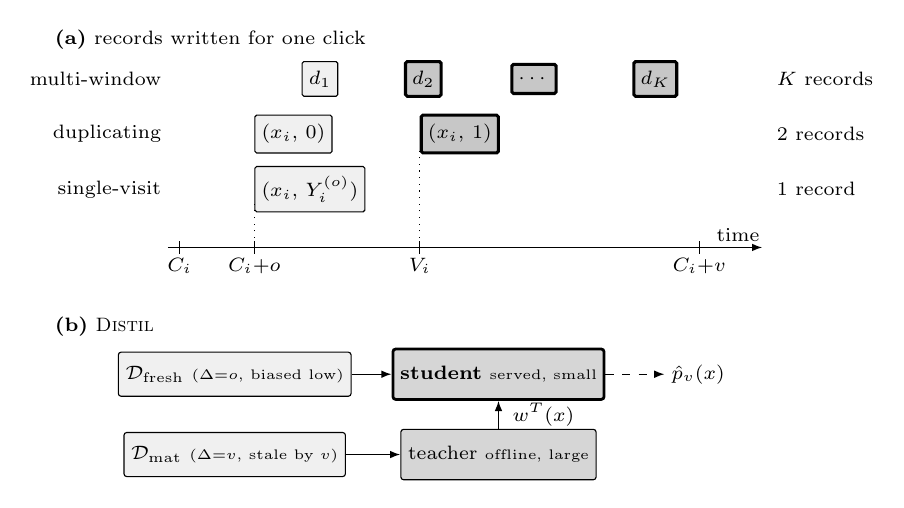
\begin{tikzpicture}[
  font=\scriptsize,
  rec/.style   = {draw, line width=0.4pt, rounded corners=0.6pt, minimum height=3.7mm,
                  inner xsep=2.4pt, fill=black!6},
  recx/.style  = {draw, line width=1.1pt, rounded corners=0.6pt, minimum height=3.7mm,
                  inner xsep=2.4pt, fill=black!22},
  tick/.style  = {draw, line width=0.4pt},
  ax/.style    = {draw, -{Latex[length=1.3mm]}, line width=0.5pt},
  lbl/.style   = {inner sep=0.8pt},
  box/.style   = {draw, line width=0.4pt, rounded corners=1pt, align=center, inner sep=2.6pt,
                  minimum height=5.6mm},
]

% =============== (a) records written for ONE click, on its own timeline ===============
\def\tC{0.00} \def\tO{0.95} \def\tV{3.05} \def\tW{7.40}
% panel (a) sits above panel (b); explanation lives in the caption, not in the artwork

\node[lbl, anchor=west] at (-1.62,3.02) {\textbf{(a)} records written for one click};

% lanes
\node[lbl, anchor=east] at (-0.20,2.52) {multi-window};
\node[rec,  anchor=west] at (1.55,2.52) {$d_1$};
\node[recx, anchor=west] at (2.85,2.52) {$d_2$};
\node[recx, anchor=west] at (4.20,2.52) {$\cdots$};
\node[recx, anchor=west] at (5.75,2.52) {$d_K$};
\node[lbl,  anchor=west] at (7.55,2.52) {$K$ records};

\node[lbl, anchor=east] at (-0.20,1.82) {duplicating};
\node[rec,  anchor=west] at (\tO,1.82) {$(x_i,\,0)$};
\node[recx, anchor=west] at (\tV,1.82) {$(x_i,\,1)$};
\node[lbl,  anchor=west] at (7.55,1.82) {2 records};

\node[lbl, anchor=east] at (-0.20,1.12) {single-visit};
\node[rec, anchor=west] at (\tO,1.12) {$(x_i,\,\Yo_i)$};
\node[lbl, anchor=west] at (7.55,1.12) {1 record};

% timeline
\draw[ax] (\tC-0.15,0.38) -- (\tW,0.38);
\foreach \p/\t in {\tC/{$C_i$}, \tO/{$C_i{+}o$}, \tV/{$V_i$}, 6.60/{$C_i{+}v$}} {
  \draw[tick] (\p,0.46) -- (\p,0.30);
  \node[lbl, below=0.5pt] at (\p,0.30) {\t};
}
\node[lbl, anchor=south east] at (\tW,0.42) {time};
\draw[dotted, line width=0.4pt] (\tO,0.50) -- (\tO,0.94);
\draw[dotted, line width=0.4pt] (\tV,0.50) -- (\tV,1.64);

% =============== (b) where DISTIL spends each pipeline ===============
\begin{scope}[yshift=-2.25cm]
  \node[lbl, anchor=west] at (-1.62,1.62) {\textbf{(b)} \textsc{Distil}};

  \node[box, fill=black!6, minimum width=2.6cm] (fresh) at (0.70,1.02)
    {$\mathcal{D}_{\text{fresh}}$ \tiny($\Delta{=}o$, biased low)};
  \node[box, fill=black!6, minimum width=2.6cm] (mat) at (0.70,0.00)
    {$\mathcal{D}_{\text{mat}}$ \tiny($\Delta{=}v$, stale by $v$)};

  \node[box, fill=black!16, minimum width=1.9cm, minimum height=6.4mm] (teach) at (4.05,0.00)
    {teacher \tiny offline, large};
  \node[box, fill=black!16, minimum width=1.9cm, minimum height=6.4mm, line width=1.0pt]
    (stud) at (4.05,1.02) {\textbf{student} \tiny served, small};

  \draw[ax] (mat.east)   -- (teach.west);
  \draw[ax] (fresh.east) -- (stud.west);
  \draw[ax] (teach.north) -- node[right=1.5pt] {$w^{T}(x)$} (stud.south);
  \draw[ax, dashed] (stud.east) -- ++(0.75,0) node[right=-1pt] {$\hat p_v(x)$};

\end{scope}

\end{tikzpicture}

\caption{(a) Records written for a single click. A compliant method writes one; duplicating and
multi-window methods write more, and thick-bordered records are the second and later visits that
violate R1. (b) \textsc{Distil} spends the matured pipeline on one offline teacher, whose soft label
retargets the single fresh record, so the served student remains single-visit}
\label{fig:pipeline}
\end{figure}

\subsection{An offline teacher on the matured pipeline}

The teacher trains only on clicks whose window has closed, $C_i + v \le T_n$ at cutoff $T_n$, under
the true label $\Yv$. It is causal by construction --- every training row's outcome was knowable at
$T_n$ --- and is itself R1/R2-compliant at $\Delta = v$. It carries two read-outs on one trunk:
\begin{equation}
p^{T}_v(x) = P(\Yv = 1 \mid x),
\qquad
w^{T}(x) = P(\Yv = 1 \mid \Yo = 0,\, x).
\end{equation}
The second is the estimand the field shares --- it is \textsc{Ulc}'s $w$, \textsc{Es-Dfm}'s
delayed-positive rate and \textsc{Ddfm}'s $z_1$ --- so comparing against \textsc{Ulc} isolates the
estimator and nothing else. The teacher is \emph{training-only} and therefore unbound by the serving
budget: that asymmetry is the whole method, and what it buys is the right to wait.

\subsection{The student}

The student writes one record per click, at age $o$, with target
\begin{equation}
\tilde{y}_i \;=\; \Yo_i + \bigl(1 - \Yo_i\bigr)\, w^{T}(x_i),
\label{eq:target}
\end{equation}
minimising binary cross-entropy against it. Equation~\eqref{eq:target} is exactly \textsc{Ulc}'s
functional form: an observed positive stays positive, an observed negative is softened by the
probability it converts later. The student never sees a second record and never sees a label that
arrived after its own release, so it satisfies R1 and R2 at the same level as \textsc{Ulc} and
\textsc{Fsiw} --- verified with the instrument of Sect.~\ref{sec:audit}, not by inspection.

Two implementation points matter and are easy to get wrong. The teacher's learning rate is fixed and
\emph{decoupled} from the student's: sharing it makes the per-arm sweep tune two models with one
scalar, which cost $0.0065$ AUC when it happened to \textsc{Fsiw}'s auxiliary in our harness. And
the teacher's soft label is withheld until it has seen a minimum number of matured rows, because a
barely-trained head asserting $0.5$ poisons a one-pass run permanently.

% =====================================================================================
\section{Experiments}\label{sec:experiments}
% =====================================================================================

\subsection{Setup}\label{sec:setup}

\noindent\textbf{Data and protocol.} Criteo-DFD~\cite{chapelle2014modeling}, 60 days of clicks with
conversion timestamps. We follow the streaming replay of~\cite{li2026twice}: pre-train on days
$[0,30)$, then stream $[30,60)$ with hourly cut-offs; at each cut-off a model consumes the records
released in that hour and then predicts every click of the next hour exactly once, scored
retrospectively against $\Yv$. Base observation age $o = 1$\,h, minibatch $8192$, AdamW, and a
learning rate selected \emph{per arm and per capacity} from
$\{10^{-6}, 2.5{\times}10^{-6}, 10^{-5}, 5{\times}10^{-5}, 2{\times}10^{-4}, 5{\times}10^{-4},
10^{-3}\}$ on a held-out chronological slice of the pre-training period. We report $v = 7$\,d, five
seeds, and paired $t$-tests over matched seeds ($^{\ast}p<0.05$, $^{\ast\ast}p<0.01$).

\noindent\textbf{Student ladder.} The served model must be small, so capacity is swept over five
rungs S0--S4 varying the categorical hash-table size ($36 \to 131{,}072$ rows, $26$\,K $\to 9.6$\,M
parameters) at a fixed embedding dimension of~8. The teacher is held at $9.5$\,M parameters
throughout, so any trend across rungs is attributable to the student. At S4 student and teacher are
within $1.3\%$ of the same parameter count, which is the cleanest available control for capacity
transfer.

\noindent\textbf{Arms.} \textsc{Oracle} labels the fresh record with $\Yv$; it is not causal and
exists only as a reference. \textsc{Fresh} trains on $\mathsf{D}_{\text{fresh}}$ uncorrected,
\textsc{Wait} on $\mathsf{D}_{\text{mat}}$. \textsc{Reweight} is \textsc{Fsiw}, \textsc{Correct} is
\textsc{Ulc}, and we include \textsc{Twice}. \textsc{Distil-NoKD} is the mandatory own-stream
ablation: the identical pipeline with the teacher trained but its label unused.

% -------------------------------------------------------------------------------------
\subsection{RQ1: which methods can be run at all?}\label{sec:audit}
% -------------------------------------------------------------------------------------

\begin{table}[t]
\caption{Training records per click, measured over a full 720-hour replay at $v=7$\,d. Counts are
per \emph{distinct click touched}, so traffic variation cannot inflate them, and the window covers
every method's longest revisit lag. $^{\dag}$\textsc{Twice}'s served tower is single-visit; its
delay head reads the conversion clock}
\label{tab:compliance}
\centering\small
\begin{tabular}{l r@{\hskip 1.1em} r@{\hskip 1.4em} c@{\hskip 1.0em} c}
\toprule
method & records/click & max & R1 & R2\\
\midrule
\multicolumn{5}{l}{\emph{admissible}}\\
\quad Fresh & 1.00 & 1 & \checkmark & \checkmark\\
\quad Wait / teacher & 1.00 & 1 & \checkmark & \checkmark\\
\quad Reweight & 1.00 & 1 & \checkmark & $\times$\\
\quad Correct & 1.00 & 1 & \checkmark & $\times$\\
\quad Twice & 1.00 & 1 & \checkmark & \checkmark$^{\dag}$\\
\midrule
\multicolumn{5}{l}{\emph{inadmissible}}\\
\quad Vanilla & 1.08 & 2 & $\times$ & $\times$\\
\quad DFM & 1.34 & 8 & $\times$ & $\times$\\
\quad ES-DFM & 1.08 & 2 & $\times$ & $\times$\\
\quad DEFUSE & 1.08 & 2 & $\times$ & $\times$\\
\quad DDFM & 1.89 & 2 & $\times$ & $\times$\\
\quad PI & 2.00 & 2 & $\times$ & $\times$\\
\quad MISS & 2.05 & 3 & $\times$ & $\times$\\
\quad IF-DFM & 2.90 & 99 & $\times$ & $\times$\\
\quad FTP & 3.00 & 3 & $\times$ & $\times$\\
\bottomrule
\end{tabular}

\end{table}


Table~\ref{tab:compliance} reports the measurement. We instrument the
feature path of every arm and count training records over a full 720-hour replay, charging only
gradient-carrying forwards so that merely \emph{scoring} a historical click is not counted. Two traps had to be
controlled, and ignoring either understates violations.\footnote{\emph{Traffic}: dividing records
consumed in an hour by clicks released in that hour conflates duplication with Criteo's diurnal
variation, since a maturity-gated stream reads clicks from $v$ ago when the rate differed --- that
way \textsc{Pi} scores a spurious $12.2$, purely because its 14-day head reads an hour carrying
${\sim}6\times$ the traffic of the denominator hour. We divide by \emph{distinct clicks touched}.
\emph{Window length}: over 48\,h \textsc{Pi} measures $1.00$ with a maximum of 1, because its two
visits are $10.5$ days apart and the second falls outside the window. We run the full stream and
score only clicks whose entire revisit horizon fits inside it.}

Nine of fourteen methods exceed one record per click. Two counts are exact integers and confirm the
instrument: \textsc{Pi} emits $2.00$, one per fixed-window head, and \textsc{Ftp} $3.00$, one per
task plus its prophet. \textsc{If-Dfm} touches one click up to 99 times. Only \textsc{Fsiw},
\textsc{Ulc} and \textsc{Twice} keep the served model single-visit.

\smallskip\noindent\textbf{The field's anchor is inadmissible.} \textsc{Vanilla} --- ``each click
trained once at base observation age $o$'' --- measures $1.08$ records per click, because matching
any published \textsc{Vanilla} row requires also emitting the late conversion as a
positive.\footnote{The fresh record alone predicts $0.107$ against a $0.227$ base rate and cannot
reproduce any published \textsc{Vanilla} log-loss; the reading that does is fresh label plus a
positive for conversions arriving after $o$.} Relative improvement reported against it is therefore
normalised by a baseline a single-visit pipeline cannot run.

\smallskip\noindent\textbf{On auxiliaries.} \textsc{Fsiw}, \textsc{Ulc} and \textsc{Twice} emit one
record for the served model but fit a \emph{separate} model on matured data, so they satisfy R1 and
sit at the boundary of R2. We read the constraint as governing the served model's training pipeline,
under which they comply; the alternative reading --- that no later-arriving conversion may inform
anything --- leaves only $\mathrm{Waiting}(\Delta)$ standing and declares the problem unsolvable
rather than selecting a method. We adopt the former and say so, because the choice determines which
methods are admissible. \textsc{Distil} is built to sit at exactly this level and no lower.

% -------------------------------------------------------------------------------------
\subsection{RQ2: performance under the constraint}\label{sec:main}
% -------------------------------------------------------------------------------------

\begin{table}[t]
\caption{AUC across the serving-capacity ladder, $v=7$\,d, five seeds. Significance on
\textsc{Distil} is against \textsc{Correct}, the strongest prior admissible method, paired over
matched seeds}
\label{tab:ladder}
\centering\small
\begin{tabular}{lrrrrr}
\toprule
student & S0 & S1 & S2 & S3 & S4\\
parameters & 26K & 46K & 115K & 645K & 9.6M\\
\midrule
\multicolumn{6}{l}{\emph{admissible: one record per click}}\\
\quad Fresh = Distil-NoKD & 0.8077 & 0.8127 & 0.8182 & 0.8227 & 0.8218\\
\quad Wait & 0.8105 & 0.8156 & 0.8212 & 0.8286 & 0.8321\\
\quad Reweight & 0.8218 & 0.8269 & 0.8334 & 0.8388 & 0.8396\\
\quad Twice & 0.8120 & 0.8217 & 0.8260 & 0.8305 & 0.8327\\
\quad Correct & 0.8276 & 0.8321 & 0.8372 & 0.8411 & 0.8411\\
\quad \textbf{Distil} & \textbf{0.8273} & \textbf{0.8328}$^{\ast}$ & \textbf{0.8377} & \textbf{0.8416}$^{\ast\ast}$ & \textbf{0.8437}$^{\ast\ast}$\\
\midrule
\multicolumn{6}{l}{\emph{inadmissible: $>1$ record per click}}\\
\quad Vanilla & 0.8222 & 0.8280 & 0.8347 & 0.8403 & 0.8412\\
\quad ES-DFM & 0.8166 & 0.8288 & 0.8357 & 0.8383 & 0.8421\\
\quad DEFUSE & 0.8171 & 0.8293 & 0.8362 & 0.8387 & 0.8423\\
\quad DDFM & 0.8275 & 0.8314 & 0.8367 & 0.8412 & 0.8436\\
\midrule
\quad Oracle \emph{(not causal)} & 0.8256 & 0.8311 & 0.8382 & 0.8438 & 0.8465\\
\bottomrule
\end{tabular}

\end{table}

Table~\ref{tab:ladder} gives the main result. \textsc{Distil} is the strongest admissible method at
every rung but S0, where it ties \textsc{Correct} ($-0.0003$, $p=0.59$); elsewhere it leads by
$+0.0008$ (S1, $p=0.018$), $+0.0004$ (S2, $p=0.089$), $+0.0005$ (S3, $p=0.005$) and $+0.0025$ (S4,
$p=3\!\times\!10^{-6}$).

The ordering of the admissible field is stable across the ladder and worth stating, because it is
not the ordering the literature reports: \textsc{Correct} $>$ \textsc{Reweight} $>$ \textsc{Twice}
$>$ \textsc{Wait} $>$ \textsc{Fresh}. \textsc{Twice}, the most recent method and the strongest
overall in its own evaluation, places fourth here --- not because the method fails but because its
CVR tower is deliberately fresh-only, so it starts from the \textsc{Fresh} floor and must climb back
with its delay head alone.

\smallskip\noindent\textbf{The gain is not capacity transfer.} \textsc{Distil-NoKD} --- the same
pipeline with the teacher trained but its label discarded --- lands exactly on \textsc{Fresh} at
every rung, as it must, since the two are the same algorithm. The distillation gain over that floor
is $+0.0189$ to $+0.0218$ AUC, significant at $p<10^{-6}$ throughout. Crucially, at S4 the student
and teacher hold the same parameter count to within $1.3\%$, and \textsc{Distil} still leads
\textsc{Correct} by its largest margin. The advantage therefore cannot be capacity flowing from a
larger model into a smaller one; it is the matured label.

% -------------------------------------------------------------------------------------
\subsection{RQ3: the effect of student capacity}\label{sec:capacity}
% -------------------------------------------------------------------------------------

\begin{figure}[t]
\centering
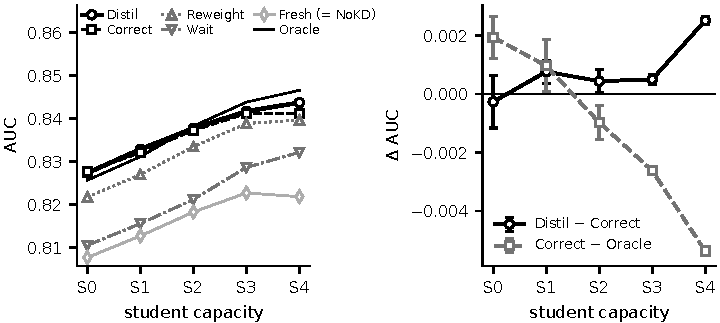
\includegraphics[width=\textwidth]{figs/fig_capacity_7d.pdf}
\caption{Left: AUC against serving capacity; all admissible methods plus the non-causal Oracle.
Right: two margins with 95\% intervals over five paired seeds. \textsc{Correct} $-$ Oracle crosses
zero between S1 and S2 --- below that, a soft-labelled admissible method beats the Oracle}
\label{fig:capacity}
\end{figure}

Fig.~\ref{fig:capacity} reports the capacity sweep; three observations follow. The secondary
metrics agree with AUC at the capacity-matched rung S4, where \textsc{Distil} reaches PR-AUC
$0.5920$ and LL $0.3496$ against \textsc{Correct}'s $0.5875$ and $0.3513$, with the non-causal
Oracle at $0.5953$ and $0.3468$.

\smallskip\noindent\textbf{The delayed-feedback penalty grows with capacity.} The recoverable gap
Oracle $-$ \textsc{Fresh} widens from $0.0179$ at S0 to $0.0247$ at S4. Small models are
intrinsically less hurt by label censoring, because they cannot exploit the resolution the missing
labels would have supplied.

\smallskip\noindent\textbf{The Oracle is not an upper bound for small students.} \textsc{Correct}
$-$ Oracle is $+0.0019$ at S0 ($p=0.006$), $+0.0010$ at S1 ($p=0.10$), then turns negative:
$-0.0010$ (S2), $-0.0026$ (S3), $-0.0054$ (S4), all significant from S2 on. Below roughly $10^{5}$
parameters a corrected soft label is \emph{better supervision than the true label}. This is
consistent with the variance account of distillation~\cite{menon2021statistical}: a soft target has
lower variance than a Bernoulli draw, and variance reduction dominates bias when capacity is scarce.
It also means an evaluation conducted only at large capacity --- as the delayed-feedback literature
does --- reports a penalty that a deployable model does not fully pay.

\smallskip\noindent\textbf{The margin over prior work widens with capacity.} \textsc{Distil} $-$
\textsc{Correct} rises from a tie at S0 to $+0.0025$ at S4. The teacher's soft label carries more
information than the small online auxiliary's, but only a student with enough capacity can absorb
the difference; at S0, with 36 hash rows, both targets are equally unrepresentable.

% -------------------------------------------------------------------------------------
\subsection{RQ4: which part of the teacher matters?}\label{sec:ablation}
% -------------------------------------------------------------------------------------

\begin{table}[t]
\caption{Teacher design, student fixed at S2. $\Delta$ is against the default teacher}
\label{tab:ablation}
\centering\small
\begin{tabular}{l r@{\hskip 1.4em} l}
\toprule
variant & AUC & $\Delta$ vs default\\
\midrule
\textsc{Distil}, teacher 9.5\,M (default) & 0.8377 & --\\
\quad teacher 57\,M & 0.8360 & $-0.0016$$^{\ast\ast}$\\
\quad teacher 60\,M & 0.8361 & $-0.0016$$^{\ast\ast}$\\
\quad teacher trains only $w$ & 0.8376 & $-0.0000$\\
\quad teacher label unused (NoKD) & 0.8182 & $-0.0194$$^{\ast\ast}$\\
\bottomrule
\end{tabular}

\end{table}

Table~\ref{tab:ablation} varies the teacher at a fixed student. Removing the soft label entirely
costs $-0.0194$, which is the whole method. Restricting the teacher to train only the head the
student consumes changes nothing ($-0.0000$), so the second read-out is free. Enlarging the teacher
from $9.5$\,M to $57$\,M or $60$\,M parameters \emph{hurts} by $-0.0016$ --- the subject of the next
section.

% -------------------------------------------------------------------------------------
\subsection{Why the teacher's margin is small on this corpus}\label{sec:headroom}
% -------------------------------------------------------------------------------------

Two comparisons are easily confused here, and separating them explains both why the teacher helps
and why enlarging it does not.

\smallskip\noindent\textbf{Teacher versus student: a large margin that shrinks with student size.}
In NE at $v=7$\,d the teacher reaches $0.7405$ against a student floor of $0.7821$ at S0 and
$0.7522$ at S4 --- headroom of $0.0416$ and $0.0117$ respectively, a factor of $3.6$. Capacity
matters at the small end, which is the end a latency-bound ranker occupies.

\smallskip\noindent\textbf{Teacher versus larger teacher: no margin at all.} Scaling past
$\sim\!9.4$\,M parameters does not help and then hurts: NE $0.7405$, $0.7454$ and $0.7489$ at
$9.4$, $57$ and $60$\,M. This is a property of the corpus. Criteo-DFD's nine categorical fields hold
$135{,}151$ distinct values in total against a table provisioned at $131{,}072$ rows \emph{per
field}, so a model at full resolution has already absorbed every input the data can distinguish and
further parameters buy access to nothing. The saturation point and the teacher's optimum coincide.
One-pass streaming compresses the ladder further: a batch-retrained variant of the same ladder spans
$0.0536$ NE from S0 to S4 where ours spans $0.0300$, and extra teacher epochs do not recover the
difference ($0.8381/0.8385/0.8345/0.8381$ AUC at 1/2/4/8 epochs).

\smallskip\noindent\textbf{An expectation, not a result.} These measurements bound teacher headroom
on a corpus whose vocabulary is ${\sim}10^{5}$ and whose saturation point is ${\sim}10^{7}$
parameters. Production catalogues and user identifiers are orders of magnitude larger, so the
saturation capacity is correspondingly higher while the student stays pinned by the serving budget;
we therefore expect a substantially larger teacher--student gap, and margin for distillation, than
the $0.0117$--$0.0416$ NE here. \emph{We do not measure this.} It is also why we report the gain
against student capacity rather than at one point: the slope, not the level, is what transfers.

% =====================================================================================
\section{Limitations}\label{sec:limits}
% =====================================================================================

One public corpus with a single conversion event, so multi-objective consolidation is motivation
rather than experiment. The constraint is one production contract among several: systems that do
support replay may use the methods we rule out, and for them our audit is a cost accounting rather
than a prohibition. Whether R2 binds auxiliary models is a reading we adopt explicitly
(Sect.~\ref{sec:audit}), not a fact about the constraint. The ladder varies table rows at fixed
embedding width; other capacity axes may differ. The extrapolation in Sect.~\ref{sec:headroom} is an
expectation grounded in a measured saturation mechanism, not a result.

% =====================================================================================
\section{Conclusion}
% =====================================================================================

Delayed-feedback methods are usually compared on accuracy alone. We added a systems constraint that
many production pipelines already impose --- one training record per click, label frozen at a fixed
wait --- and measured who satisfies it. Nine of fourteen published methods do not, including the
baseline the field normalises against. Among those that do, spending the matured-label pipeline on a
single offline teacher and distilling it into a single-visit student is the strongest option we
find, and at equal student--teacher capacity the gain is attributable to the teacher's matured
labels rather than to its size. The capacity sweep also shows that the delayed-feedback penalty, and
the value of a corrected label, both depend strongly on the size of the served model --- to the
point that below $10^{5}$ parameters a corrected soft label beats the true one. Evaluating at a
single capacity, as the literature does, hides this.

\bibliographystyle{splncs04}
\bibliography{refs}

\end{document}
